\PassOptionsToPackage{unicode=true}{hyperref} % options for packages loaded elsewhere
\PassOptionsToPackage{hyphens}{url}
%
\documentclass[11pt,ignorenonframetext,]{beamer}
\usepackage{pgfpages}
\setbeamertemplate{caption}[numbered]
\setbeamertemplate{caption label separator}{: }
\setbeamercolor{caption name}{fg=normal text.fg}
\beamertemplatenavigationsymbolsempty
% Prevent slide breaks in the middle of a paragraph:
\widowpenalties 1 10000
\raggedbottom
\setbeamertemplate{part page}{
\centering
\begin{beamercolorbox}[sep=16pt,center]{part title}
  \usebeamerfont{part title}\insertpart\par
\end{beamercolorbox}
}
\setbeamertemplate{section page}{
\centering
\begin{beamercolorbox}[sep=12pt,center]{part title}
  \usebeamerfont{section title}\insertsection\par
\end{beamercolorbox}
}
\setbeamertemplate{subsection page}{
\centering
\begin{beamercolorbox}[sep=8pt,center]{part title}
  \usebeamerfont{subsection title}\insertsubsection\par
\end{beamercolorbox}
}
\AtBeginPart{
  \frame{\partpage}
}
\AtBeginSection{
  \ifbibliography
  \else
    \frame{\sectionpage}
  \fi
}
\AtBeginSubsection{
  \frame{\subsectionpage}
}
\usepackage{lmodern}
\usepackage{amssymb,amsmath}
\usepackage{ifxetex,ifluatex}
\usepackage{fixltx2e} % provides \textsubscript
\ifnum 0\ifxetex 1\fi\ifluatex 1\fi=0 % if pdftex
  \usepackage[T1]{fontenc}
  \usepackage[utf8]{inputenc}
  \usepackage{textcomp} % provides euro and other symbols
\else % if luatex or xelatex
  \usepackage{unicode-math}
  \defaultfontfeatures{Ligatures=TeX,Scale=MatchLowercase}
\fi
\usetheme[]{metropolis}
% use upquote if available, for straight quotes in verbatim environments
\IfFileExists{upquote.sty}{\usepackage{upquote}}{}
% use microtype if available
\IfFileExists{microtype.sty}{%
\usepackage[]{microtype}
\UseMicrotypeSet[protrusion]{basicmath} % disable protrusion for tt fonts
}{}
\IfFileExists{parskip.sty}{%
\usepackage{parskip}
}{% else
\setlength{\parindent}{0pt}
\setlength{\parskip}{6pt plus 2pt minus 1pt}
}
\usepackage{hyperref}
\hypersetup{
            pdftitle={Lecture 19},
            pdfauthor={Colin Rundel},
            pdfborder={0 0 0},
            breaklinks=true}
\urlstyle{same}  % don't use monospace font for urls
\newif\ifbibliography
\usepackage{color}
\usepackage{fancyvrb}
\newcommand{\VerbBar}{|}
\newcommand{\VERB}{\Verb[commandchars=\\\{\}]}
\DefineVerbatimEnvironment{Highlighting}{Verbatim}{commandchars=\\\{\}}
% Add ',fontsize=\small' for more characters per line
\newenvironment{Shaded}{}{}
\newcommand{\AlertTok}[1]{\textcolor[rgb]{1.00,0.00,0.00}{\textbf{#1}}}
\newcommand{\AnnotationTok}[1]{\textcolor[rgb]{0.38,0.63,0.69}{\textbf{\textit{#1}}}}
\newcommand{\AttributeTok}[1]{\textcolor[rgb]{0.49,0.56,0.16}{#1}}
\newcommand{\BaseNTok}[1]{\textcolor[rgb]{0.25,0.63,0.44}{#1}}
\newcommand{\BuiltInTok}[1]{#1}
\newcommand{\CharTok}[1]{\textcolor[rgb]{0.25,0.44,0.63}{#1}}
\newcommand{\CommentTok}[1]{\textcolor[rgb]{0.38,0.63,0.69}{\textit{#1}}}
\newcommand{\CommentVarTok}[1]{\textcolor[rgb]{0.38,0.63,0.69}{\textbf{\textit{#1}}}}
\newcommand{\ConstantTok}[1]{\textcolor[rgb]{0.53,0.00,0.00}{#1}}
\newcommand{\ControlFlowTok}[1]{\textcolor[rgb]{0.00,0.44,0.13}{\textbf{#1}}}
\newcommand{\DataTypeTok}[1]{\textcolor[rgb]{0.56,0.13,0.00}{#1}}
\newcommand{\DecValTok}[1]{\textcolor[rgb]{0.25,0.63,0.44}{#1}}
\newcommand{\DocumentationTok}[1]{\textcolor[rgb]{0.73,0.13,0.13}{\textit{#1}}}
\newcommand{\ErrorTok}[1]{\textcolor[rgb]{1.00,0.00,0.00}{\textbf{#1}}}
\newcommand{\ExtensionTok}[1]{#1}
\newcommand{\FloatTok}[1]{\textcolor[rgb]{0.25,0.63,0.44}{#1}}
\newcommand{\FunctionTok}[1]{\textcolor[rgb]{0.02,0.16,0.49}{#1}}
\newcommand{\ImportTok}[1]{#1}
\newcommand{\InformationTok}[1]{\textcolor[rgb]{0.38,0.63,0.69}{\textbf{\textit{#1}}}}
\newcommand{\KeywordTok}[1]{\textcolor[rgb]{0.00,0.44,0.13}{\textbf{#1}}}
\newcommand{\NormalTok}[1]{#1}
\newcommand{\OperatorTok}[1]{\textcolor[rgb]{0.40,0.40,0.40}{#1}}
\newcommand{\OtherTok}[1]{\textcolor[rgb]{0.00,0.44,0.13}{#1}}
\newcommand{\PreprocessorTok}[1]{\textcolor[rgb]{0.74,0.48,0.00}{#1}}
\newcommand{\RegionMarkerTok}[1]{#1}
\newcommand{\SpecialCharTok}[1]{\textcolor[rgb]{0.25,0.44,0.63}{#1}}
\newcommand{\SpecialStringTok}[1]{\textcolor[rgb]{0.73,0.40,0.53}{#1}}
\newcommand{\StringTok}[1]{\textcolor[rgb]{0.25,0.44,0.63}{#1}}
\newcommand{\VariableTok}[1]{\textcolor[rgb]{0.10,0.09,0.49}{#1}}
\newcommand{\VerbatimStringTok}[1]{\textcolor[rgb]{0.25,0.44,0.63}{#1}}
\newcommand{\WarningTok}[1]{\textcolor[rgb]{0.38,0.63,0.69}{\textbf{\textit{#1}}}}
\usepackage{longtable,booktabs}
\usepackage{caption}
% These lines are needed to make table captions work with longtable:
\makeatletter
\def\fnum@table{\tablename~\thetable}
\makeatother
\setlength{\emergencystretch}{3em}  % prevent overfull lines
\providecommand{\tightlist}{%
  \setlength{\itemsep}{0pt}\setlength{\parskip}{0pt}}
\setcounter{secnumdepth}{0}

% set default figure placement to htbp
\makeatletter
\def\fps@figure{htbp}
\makeatother

\usepackage{geometry}
\usepackage{graphicx}

\usepackage{bbold}
\usepackage{lmodern}


\usepackage{url}		% produces hyperlinks

\usepackage{colortbl}	% allows for color usage in tables
\usepackage{multirow}	% allows for rows that span multiple rows in tables

\usepackage{color}          	% gives color options
\usepackage{xcolor}		% this package has a variety of color options

\usepackage{multicol}
\usepackage{textcomp}

\usepackage{setspace}
\usepackage{changepage}
\usepackage{isotope}

\singlespacing

\def\begincol{\begin{column}}
\def\endcol{\end{column}}

\def\begincols{\begin{columns}}
\def\endcols{\end{columns}}

%%%%%%%%%%%%%%%%
% Small code output
%%%%%%%%%%%%%%%%

%% change fontsize of R code

\makeatletter
\@ifundefined{Shaded}{\newenvironment{Shaded}{}{}}{}
\makeatother


\let\oldShaded\Shaded
\let\endoldShaded\endShaded
\renewenvironment{Shaded}{\footnotesize\begin{spacing}{0.9}\oldShaded}{\endoldShaded\end{spacing}}

%% change fontsize of output
\let\oldverbatim\verbatim
\let\endoldverbatim\endverbatim
\renewenvironment{verbatim}{\footnotesize\begin{spacing}{0.9}\oldverbatim}{\endoldverbatim\end{spacing}}


\newcommand{\tinyoutput}{
  \renewenvironment{Shaded}{\tiny\begin{spacing}{0.9}\oldShaded}{\endoldShaded\end{spacing}}
  \renewenvironment{verbatim}{\tiny\begin{spacing}{0.9}\oldverbatim}{\endoldverbatim\end{spacing}}
}

\newcommand{\scriptoutput}{
  \renewenvironment{Shaded}{\scriptsize\begin{spacing}{0.9}\oldShaded}{\endoldShaded\end{spacing}}
  \renewenvironment{verbatim}{\scriptsize\begin{spacing}{0.9}\oldverbatim}{\endoldverbatim\end{spacing}}
}

\newcommand{\footnoteoutput}{
  \renewenvironment{Shaded}{\footnotesize\begin{spacing}{0.9}\oldShaded}{\endoldShaded\end{spacing}}
  \renewenvironment{verbatim}{\footnotesize\begin{spacing}{0.9}\oldverbatim}{\endoldverbatim\end{spacing}}
}

%\newcommand{\verbatimfont}[1]{\renewcommand{\verbatim@font}{\ttfamily#1}}


%%%%%%%%%%%%%%%%
% Custom Colors
%%%%%%%%%%%%%%%%

\definecolor{redhl}{rgb}{0.98,0.29,0.28}
\definecolor{yellowhl}{rgb}{0.98,0.87,0.28}


\xdefinecolor{oiBlue}{rgb}{0.15, 0.35, 0.55}
\xdefinecolor{gray}{rgb}{0.5, 0.5, 0.5}
\xdefinecolor{darkGray}{rgb}{0.3, 0.3, 0.3}
\xdefinecolor{darkerGray}{rgb}{0.2, 0.2, 0.2}
\xdefinecolor{rubineRed}{rgb}{0.89,0,0.30}
\xdefinecolor{linkCol}{rgb}{0.11,0.49,0.95}	
\xdefinecolor{irishGreen}{rgb}{0,0.60,0}	
\xdefinecolor{darkturquoise}{rgb}{0.44, 0.58, 0.86}
\definecolor{lightGreen}{rgb}{0.533,0.765,0.42}
%\xdefinecolor{hlblue}{rgb}{0.051,0.65,1}
\xdefinecolor{hlblue}{rgb}{ 0.055, 0.639, 0.831}
\definecolor{light}{rgb}{.337,.608,.741}
\definecolor{dark}{rgb}{.337,.608,.741}

\definecolor{cpink}{rgb}{0.93, 0.23, 0.51}

%%%%%%%%%%%%%%%%
% Custom Commands
%%%%%%%%%%%%%%%%

% text colors
\newcommand{\red}[1]{\textit{\textcolor{rubineRed}{#1}}}
\newcommand{\orange}[1]{\textit{\textcolor{orange}{#1}}}
\newcommand{\pink}[1]{\textit{\textcolor{rubineRed!90!white!50}{#1}}}
\newcommand{\green}[1]{\textit{\textcolor{irishGreen}{#1}}}
\newcommand{\blue}[1]{\textit{\textcolor{darkturquoise}{#1}}}
\newcommand{\light}[1]{\textcolor{light}{\textbf{#1}}}
\newcommand{\dark}[1]{\textcolor{dark}{#1}}
\newcommand{\gray}[1]{\textcolor{gray}{#1}}


% mail
\newcommand{\mail}[1]{\href{mailto:#1}{\textit{\textcolor{linkCol}{#1}}}}

% highlighting: hl, hlGr, mathhl
\newcommand{\hl}[1]{\textit{\textcolor{hlblue}{#1}}}
\newcommand{\hlGr}[1]{\textit{\textcolor{lightGreen}{#1}}}
\newcommand{\hlRd}[1]{\textit{\textcolor{rubineRed}{#1}}}
\newcommand{\mathhl}[1]{\textcolor{hlblue}{\ensuremath{#1}}}
\newcommand{\hlr}[1]{\fcolorbox{redhl}{white}{$\displaystyle #1$}}
\newcommand{\hly}[1]{\fcolorbox{yellowhl}{white}{$\displaystyle #1$}}


\newcommand{\vvfill}{\vskip0pt plus 1filll}

\DeclareMathOperator*{\argmin}{arg\,min}
\DeclareMathOperator*{\argmax}{arg\,max}

\title{Lecture 19}
\providecommand{\subtitle}[1]{}
\subtitle{Spatial GLM + Point Reference Spatial Data}
\author{Colin Rundel}
\date{11/09/2017}

\begin{document}
\frame{\titlepage}

\hypertarget{spatial-glm-models}{%
\section{Spatial GLM Models}\label{spatial-glm-models}}

\begin{frame}{Scottish Lip Cancer Data}
\protect\hypertarget{scottish-lip-cancer-data}{}

\begin{center}\includegraphics[width=\textwidth]{Lec19_files/figure-beamer/unnamed-chunk-1-1} \end{center}

\end{frame}

\begin{frame}{}
\protect\hypertarget{section}{}

\begin{center}\includegraphics[width=\textwidth]{Lec19_files/figure-beamer/unnamed-chunk-2-1} \end{center}

\end{frame}

\begin{frame}{Neighborhood / weight matrix}
\protect\hypertarget{neighborhood-weight-matrix}{}

\vspace{-4mm}

\begin{center}\includegraphics[width=0.5\textwidth]{Lec19_files/figure-beamer/unnamed-chunk-3-1} \end{center}

\end{frame}

\begin{frame}[fragile]{Moran's I}
\protect\hypertarget{morans-i}{}

\scriptoutput

\begin{Shaded}
\begin{Highlighting}[]
\NormalTok{spdep}\OperatorTok{::}\KeywordTok{moran.test}\NormalTok{(lip_cancer}\OperatorTok{$}\NormalTok{Observed, listw)}
\CommentTok{## }
\CommentTok{##  Moran I test under randomisation}
\CommentTok{## }
\CommentTok{## data:  lip_cancer$Observed  }
\CommentTok{## weights: listw    }
\CommentTok{## }
\CommentTok{## Moran I statistic standard deviate = 4.5416, p-value = 2.792e-06}
\CommentTok{## alternative hypothesis: greater}
\CommentTok{## sample estimates:}
\CommentTok{## Moran I statistic       Expectation          Variance }
\CommentTok{##       0.311975396      -0.018181818       0.005284831}

\NormalTok{spdep}\OperatorTok{::}\KeywordTok{moran.test}\NormalTok{(lip_cancer}\OperatorTok{$}\NormalTok{Observed }\OperatorTok{/}\StringTok{ }\NormalTok{lip_cancer}\OperatorTok{$}\NormalTok{Expected, listw)}
\CommentTok{## }
\CommentTok{##  Moran I test under randomisation}
\CommentTok{## }
\CommentTok{## data:  lip_cancer$Observed/lip_cancer$Expected  }
\CommentTok{## weights: listw    }
\CommentTok{## }
\CommentTok{## Moran I statistic standard deviate = 8.2916, p-value < 2.2e-16}
\CommentTok{## alternative hypothesis: greater}
\CommentTok{## sample estimates:}
\CommentTok{## Moran I statistic       Expectation          Variance }
\CommentTok{##       0.589795225      -0.018181818       0.005376506}
\end{Highlighting}
\end{Shaded}

\end{frame}

\begin{frame}[fragile]{GLM}
\protect\hypertarget{glm}{}

\scriptoutput

\begin{Shaded}
\begin{Highlighting}[]
\NormalTok{l =}\StringTok{ }\KeywordTok{glm}\NormalTok{(Observed }\OperatorTok{~}\StringTok{ }\KeywordTok{offset}\NormalTok{(}\KeywordTok{log}\NormalTok{(Expected)) }\OperatorTok{+}\StringTok{ }\NormalTok{pcaff, }
        \DataTypeTok{family=}\StringTok{"poisson"}\NormalTok{, }\DataTypeTok{data=}\NormalTok{lip_cancer)}

\KeywordTok{summary}\NormalTok{(l)}
\CommentTok{## }
\CommentTok{## Call:}
\CommentTok{## glm(formula = Observed ~ offset(log(Expected)) + pcaff, family = "poisson", }
\CommentTok{##     data = lip_cancer)}
\CommentTok{## }
\CommentTok{## Deviance Residuals: }
\CommentTok{##     Min       1Q   Median       3Q      Max  }
\CommentTok{## -4.7632  -1.2156   0.0967   1.3362   4.7130  }
\CommentTok{## }
\CommentTok{## Coefficients:}
\CommentTok{##              Estimate Std. Error z value Pr(>|z|)    }
\CommentTok{## (Intercept) -0.542268   0.069525   -7.80 6.21e-15 ***}
\CommentTok{## pcaff        0.073732   0.005956   12.38  < 2e-16 ***}
\CommentTok{## ---}
\CommentTok{## Signif. codes:  0 '***' 0.001 '**' 0.01 '*' 0.05 '.' 0.1 ' ' 1}
\CommentTok{## }
\CommentTok{## (Dispersion parameter for poisson family taken to be 1)}
\CommentTok{## }
\CommentTok{##     Null deviance: 380.73  on 55  degrees of freedom}
\CommentTok{## Residual deviance: 238.62  on 54  degrees of freedom}
\CommentTok{## AIC: 450.6}
\CommentTok{## }
\CommentTok{## Number of Fisher Scoring iterations: 5}
\end{Highlighting}
\end{Shaded}

\end{frame}

\begin{frame}{GLM Fit}
\protect\hypertarget{glm-fit}{}

\begin{center}\includegraphics[width=\textwidth]{Lec19_files/figure-beamer/unnamed-chunk-6-1} \end{center}

\end{frame}

\begin{frame}{GLM Fit}
\protect\hypertarget{glm-fit-1}{}

\begin{center}\includegraphics[width=\textwidth]{Lec19_files/figure-beamer/unnamed-chunk-7-1} \end{center}

\end{frame}

\begin{frame}{GLM Residuals}
\protect\hypertarget{glm-residuals}{}

\begin{center}\includegraphics[width=\textwidth]{Lec19_files/figure-beamer/unnamed-chunk-8-1} \end{center}

\end{frame}

\begin{frame}[fragile]{Model Results}
\protect\hypertarget{model-results}{}

\begin{Shaded}
\begin{Highlighting}[]
\CommentTok{#RMSE}
\NormalTok{lip_cancer}\OperatorTok{$}\NormalTok{glm_resid }\OperatorTok\StringTok{ }\NormalTok{.}\OperatorTok{^}\DecValTok{2} \OperatorTok\StringTok{ }\KeywordTok{mean}\NormalTok{() }\OperatorTok\StringTok{ }\KeywordTok{sqrt}\NormalTok{()}
\CommentTok{## [1] 7.480889}

\CommentTok{#Moran's I}
\NormalTok{spdep}\OperatorTok{::}\KeywordTok{moran.test}\NormalTok{(lip_cancer}\OperatorTok{$}\NormalTok{glm_resid, listw)}
\CommentTok{## }
\CommentTok{##  Moran I test under randomisation}
\CommentTok{## }
\CommentTok{## data:  lip_cancer$glm_resid  }
\CommentTok{## weights: listw    }
\CommentTok{## }
\CommentTok{## Moran I statistic standard deviate = 4.8186, p-value = 7.228e-07}
\CommentTok{## alternative hypothesis: greater}
\CommentTok{## sample estimates:}
\CommentTok{## Moran I statistic       Expectation          Variance }
\CommentTok{##       0.333403223      -0.018181818       0.005323717}
\end{Highlighting}
\end{Shaded}

\end{frame}

\begin{frame}[t]{A hierachical model for lip cancer}
\protect\hypertarget{a-hierachical-model-for-lip-cancer}{}

We have observed counts of lip cancer for 56 districts in Scotland. Let
\(y_i\) represent the number of lip cancer for district \(i\).

\[\begin{aligned}
y_i &\sim \text{Poisson}(\lambda_i) \\
\\
\log(\lambda_i) &= \log(E_i) + x_i \beta + \omega_i \\
\\
\symbf{\omega} &\sim \mathcal{N}(\symbf{0},~\sigma^2(\symbf{D}-\phi\,\symbf{W})^{-1})
\end{aligned}\]

where \(E_i\) is the expected counts for each region (and serves as an
offet).

\end{frame}

\begin{frame}[fragile]{Data prep \& CAR model}
\protect\hypertarget{data-prep-car-model}{}

\scriptoutput

\begin{Shaded}
\begin{Highlighting}[]
\NormalTok{D =}\StringTok{ }\KeywordTok{diag}\NormalTok{(}\KeywordTok{rowSums}\NormalTok{(W))}
\NormalTok{X =}\StringTok{ }\KeywordTok{model.matrix}\NormalTok{(}\OperatorTok{~}\KeywordTok{scale}\NormalTok{(lip_cancer}\OperatorTok{$}\NormalTok{pcaff))}
\NormalTok{log_offset =}\StringTok{ }\KeywordTok{log}\NormalTok{(lip_cancer}\OperatorTok{$}\NormalTok{Expected)}
\NormalTok{y =}\StringTok{ }\NormalTok{lip_cancer}\OperatorTok{$}\NormalTok{Observed}
\end{Highlighting}
\end{Shaded}

\begin{Shaded}
\begin{Highlighting}[]
\NormalTok{car_model =}\StringTok{ "model\{}
\StringTok{  for(i in 1:length(y)) \{}
\StringTok{    y[i] ~ dpois(lambda[i])}
\StringTok{    y_pred[i] ~ dpois(lambda[i])}
\StringTok{    log(lambda[i]) = log_offset[i] + X[i,] %*% beta + omega[i]}
\StringTok{  \}}

\StringTok{  for(i in 1:2) \{}
\StringTok{    beta[i] ~ dnorm(0,1)}
\StringTok{  \}}

\StringTok{  omega ~ dmnorm(rep(0,length(y)), tau * (D - phi*W))}
\StringTok{  sigma2 = 1/tau}
\StringTok{  tau ~ dgamma(2, 2)}
\StringTok{  phi ~ dunif(0,0.99)}
\StringTok{\}"}
\end{Highlighting}
\end{Shaded}

\end{frame}

\begin{frame}{CAR Results}
\protect\hypertarget{car-results}{}

\begin{center}\includegraphics[width=\textwidth]{Lec19_files/figure-beamer/unnamed-chunk-13-1} \end{center}

\end{frame}

\begin{frame}{}
\protect\hypertarget{section-1}{}

\begin{center}\includegraphics[width=\textwidth]{Lec19_files/figure-beamer/unnamed-chunk-14-1} \end{center}

\end{frame}

\begin{frame}{CAR Predictions}
\protect\hypertarget{car-predictions}{}

\begin{center}\includegraphics[width=\textwidth]{Lec19_files/figure-beamer/unnamed-chunk-15-1} \end{center}

\end{frame}

\begin{frame}{CAR Predictions}
\protect\hypertarget{car-predictions-1}{}

\begin{center}\includegraphics[width=\textwidth]{Lec19_files/figure-beamer/unnamed-chunk-16-1} \end{center}

\end{frame}

\begin{frame}{CAR Residuals}
\protect\hypertarget{car-residuals}{}

\begin{center}\includegraphics[width=\textwidth]{Lec19_files/figure-beamer/unnamed-chunk-17-1} \end{center}

\end{frame}

\begin{frame}[fragile,t]{CAR Results}
\protect\hypertarget{car-results-1}{}

\begin{Shaded}
\begin{Highlighting}[]
\CommentTok{#RMSE}
\NormalTok{lip_cancer}\OperatorTok{$}\NormalTok{car_resid }\OperatorTok\StringTok{ }\NormalTok{.}\OperatorTok{^}\DecValTok{2} \OperatorTok\StringTok{ }\KeywordTok{mean}\NormalTok{() }\OperatorTok\StringTok{ }\KeywordTok{sqrt}\NormalTok{()}
\CommentTok{## [1] 1.586241}

\CommentTok{#Moran's I}
\NormalTok{spdep}\OperatorTok{::}\KeywordTok{moran.test}\NormalTok{(lip_cancer}\OperatorTok{$}\NormalTok{car_resid, listw)}
\CommentTok{## }
\CommentTok{##  Moran I test under randomisation}
\CommentTok{## }
\CommentTok{## data:  lip_cancer$car_resid  }
\CommentTok{## weights: listw    }
\CommentTok{## }
\CommentTok{## Moran I statistic standard deviate = 1.0633, p-value = 0.1438}
\CommentTok{## alternative hypothesis: greater}
\CommentTok{## sample estimates:}
\CommentTok{## Moran I statistic       Expectation          Variance }
\CommentTok{##       0.061804482      -0.018181818       0.005658742}
\end{Highlighting}
\end{Shaded}

\end{frame}

\begin{frame}[fragile]{Intrinsic Autoregressive Model}
\protect\hypertarget{intrinsic-autoregressive-model}{}

\begin{Shaded}
\begin{Highlighting}[]
\NormalTok{iar_model =}\StringTok{ "model\{}
\StringTok{  for(i in 1:length(y)) \{}
\StringTok{    y[i] ~ dpois(lambda[i])}
\StringTok{    y_pred[i] ~ dpois(lambda[i])}
\StringTok{    log(lambda[i]) = log_offset[i] + X[i,] %*% beta + omega[i]}
\StringTok{  \}}

\StringTok{  for(i in 1:2) \{}
\StringTok{    beta[i] ~ dnorm(0,1)}
\StringTok{  \}}

\StringTok{  omega_free ~ dmnorm(rep(0,length(y)), tau * (D - W))}
\StringTok{  omega = omega_free - mean(omega_free)}
\StringTok{  sigma2 = 1/tau}
\StringTok{  tau ~ dgamma(2, 2)}
\StringTok{\}"}
\end{Highlighting}
\end{Shaded}

\end{frame}

\begin{frame}{Model Parameters}
\protect\hypertarget{model-parameters}{}

\begin{center}\includegraphics[width=\textwidth]{Lec19_files/figure-beamer/unnamed-chunk-21-1} \end{center}

\end{frame}

\begin{frame}{Predictions}
\protect\hypertarget{predictions}{}

\begin{center}\includegraphics[width=\textwidth]{Lec19_files/figure-beamer/unnamed-chunk-22-1} \end{center}

\end{frame}

\begin{frame}{Residuals}
\protect\hypertarget{residuals}{}

\begin{center}\includegraphics[width=\textwidth]{Lec19_files/figure-beamer/unnamed-chunk-23-1} \end{center}

\end{frame}

\begin{frame}[fragile,t]{IAR Results}
\protect\hypertarget{iar-results}{}

\begin{Shaded}
\begin{Highlighting}[]
\CommentTok{#RMSE}
\NormalTok{lip_cancer}\OperatorTok{$}\NormalTok{iar_resid }\OperatorTok\StringTok{ }\NormalTok{.}\OperatorTok{^}\DecValTok{2} \OperatorTok\StringTok{ }\KeywordTok{mean}\NormalTok{() }\OperatorTok\StringTok{ }\KeywordTok{sqrt}\NormalTok{()}
\CommentTok{## [1] 4.473069}

\CommentTok{#Moran's I}
\NormalTok{spdep}\OperatorTok{::}\KeywordTok{moran.test}\NormalTok{(lip_cancer}\OperatorTok{$}\NormalTok{iar_resid, listw)}
\CommentTok{## }
\CommentTok{##  Moran I test under randomisation}
\CommentTok{## }
\CommentTok{## data:  lip_cancer$iar_resid  }
\CommentTok{## weights: listw    }
\CommentTok{## }
\CommentTok{## Moran I statistic standard deviate = 2.6377, p-value = 0.004174}
\CommentTok{## alternative hypothesis: greater}
\CommentTok{## sample estimates:}
\CommentTok{## Moran I statistic       Expectation          Variance }
\CommentTok{##       0.175216401      -0.018181818       0.005375965}
\end{Highlighting}
\end{Shaded}

\end{frame}

\begin{frame}[fragile]{Intrinsic Autoregressive Model - Reparameterized}
\protect\hypertarget{intrinsic-autoregressive-model---reparameterized}{}

\begin{Shaded}
\begin{Highlighting}[]
\NormalTok{iar_model2 =}\StringTok{ "model\{}
\StringTok{  for(i in 1:length(y)) \{}
\StringTok{    y[i] ~ dpois(lambda[i])}
\StringTok{    y_pred[i] ~ dpois(lambda[i])}
\StringTok{    log(lambda[i]) = log_offset[i] + X[i,] %*% beta + sigma * omega[i]}
\StringTok{  \}}

\StringTok{  for(i in 1:2) \{}
\StringTok{    beta[i] ~ dnorm(0,1)}
\StringTok{  \}}

\StringTok{  omega_free ~ dmnorm(rep(0,length(y)), (D - W))}
\StringTok{  omega = omega_free - mean(omega_free)}
\StringTok{  sigma2 = 1/tau}
\StringTok{  sigma = sqrt(sigma2)}
\StringTok{  tau ~ dgamma(2, 2)}
\StringTok{\}"}
\end{Highlighting}
\end{Shaded}

\end{frame}

\begin{frame}{IAR(2) Parameters}
\protect\hypertarget{iar2-parameters}{}

\begin{center}\includegraphics[width=\textwidth]{Lec19_files/figure-beamer/unnamed-chunk-27-1} \end{center}

\end{frame}

\begin{frame}{Predictions}
\protect\hypertarget{predictions-1}{}

\begin{center}\includegraphics[width=\textwidth]{Lec19_files/figure-beamer/unnamed-chunk-28-1} \end{center}

\end{frame}

\begin{frame}{Predictions (cont.)}
\protect\hypertarget{predictions-cont.}{}

\begin{center}\includegraphics[width=\textwidth]{Lec19_files/figure-beamer/unnamed-chunk-29-1} \end{center}

\end{frame}

\begin{frame}{Residuals}
\protect\hypertarget{residuals-1}{}

\begin{center}\includegraphics[width=\textwidth]{Lec19_files/figure-beamer/unnamed-chunk-30-1} \end{center}

\end{frame}

\begin{frame}[fragile,t]{IAR(2) Results}
\protect\hypertarget{iar2-results}{}

\begin{Shaded}
\begin{Highlighting}[]
\CommentTok{#RMSE}
\NormalTok{lip_cancer}\OperatorTok{$}\NormalTok{iar2_resid }\OperatorTok\StringTok{ }\NormalTok{.}\OperatorTok{^}\DecValTok{2} \OperatorTok\StringTok{ }\KeywordTok{mean}\NormalTok{() }\OperatorTok\StringTok{ }\KeywordTok{sqrt}\NormalTok{()}
\CommentTok{## [1] 1.654235}

\CommentTok{#Moran's I}
\NormalTok{spdep}\OperatorTok{::}\KeywordTok{moran.test}\NormalTok{(lip_cancer}\OperatorTok{$}\NormalTok{iar2_resid, listw)}
\CommentTok{## }
\CommentTok{##  Moran I test under randomisation}
\CommentTok{## }
\CommentTok{## data:  lip_cancer$iar2_resid  }
\CommentTok{## weights: listw    }
\CommentTok{## }
\CommentTok{## Moran I statistic standard deviate = 0.39186, p-value = 0.3476}
\CommentTok{## alternative hypothesis: greater}
\CommentTok{## sample estimates:}
\CommentTok{## Moran I statistic       Expectation          Variance }
\CommentTok{##       0.011188088      -0.018181818       0.005617437}
\end{Highlighting}
\end{Shaded}

\end{frame}

\begin{frame}{Overall Results}
\protect\hypertarget{overall-results}{}

\begin{longtable}[]{@{}lrr@{}}
\toprule
model & rmse & moran\tabularnewline
\midrule
\endhead
glm & 7.4809 & 0.3334\tabularnewline
car & 1.5862 & 0.0618\tabularnewline
iar & 4.4731 & 0.1752\tabularnewline
iar2 & 1.6542 & 0.0112\tabularnewline
\bottomrule
\end{longtable}

\end{frame}

\hypertarget{point-referenced-data}{%
\section{Point Referenced Data}\label{point-referenced-data}}

\begin{frame}{Example - PM2.5 from CSN}
\protect\hypertarget{example---pm2.5-from-csn}{}

The Chemical Speciation Network are a series of air quality monitors run
by EPA (221 locations in 2007). We'll look at a subset of the data from
Nov 11th, 2007 (n=191) for just PM2.5.

\begin{center}\includegraphics[width=\textwidth]{Lec19_files/figure-beamer/unnamed-chunk-33-1} \end{center}

\end{frame}

\begin{frame}[fragile]{}
\protect\hypertarget{section-2}{}

\begin{Shaded}
\begin{Highlighting}[]
\NormalTok{csn}
\CommentTok{## # A tibble: 191 x 5}
\CommentTok{##        site longitude latitude date                 pm25}
\CommentTok{##       <int>     <dbl>    <dbl> <dttm>              <dbl>}
\CommentTok{##  1 10730023     -86.8     33.6 2007-11-14 00:00:00  19.4}
\CommentTok{##  2 10732003     -86.9     33.5 2007-11-14 00:00:00  26.4}
\CommentTok{##  3 10890014     -86.6     34.7 2007-11-14 00:00:00  13.4}
\CommentTok{##  4 11011002     -86.3     32.4 2007-11-14 00:00:00  19.7}
\CommentTok{##  5 11130001     -85.0     32.5 2007-11-14 00:00:00  22.6}
\CommentTok{##  6 40139997    -112.      33.5 2007-11-14 00:00:00  12.3}
\CommentTok{##  7 40191028    -111.      32.3 2007-11-14 00:00:00   7.2}
\CommentTok{##  8 51190007     -92.3     34.8 2007-11-14 00:00:00  12.7}
\CommentTok{##  9 60070002    -122.      39.8 2007-11-14 00:00:00  10  }
\CommentTok{## 10 60190008    -120.      36.8 2007-11-14 00:00:00  32.3}
\CommentTok{## # ... with 181 more rows}
\end{Highlighting}
\end{Shaded}

\end{frame}

\begin{frame}{Aside - Splines}
\protect\hypertarget{aside---splines}{}

\begin{center}
\includegraphics[width=0.49\textwidth]{figs/spline1.png}
$~$
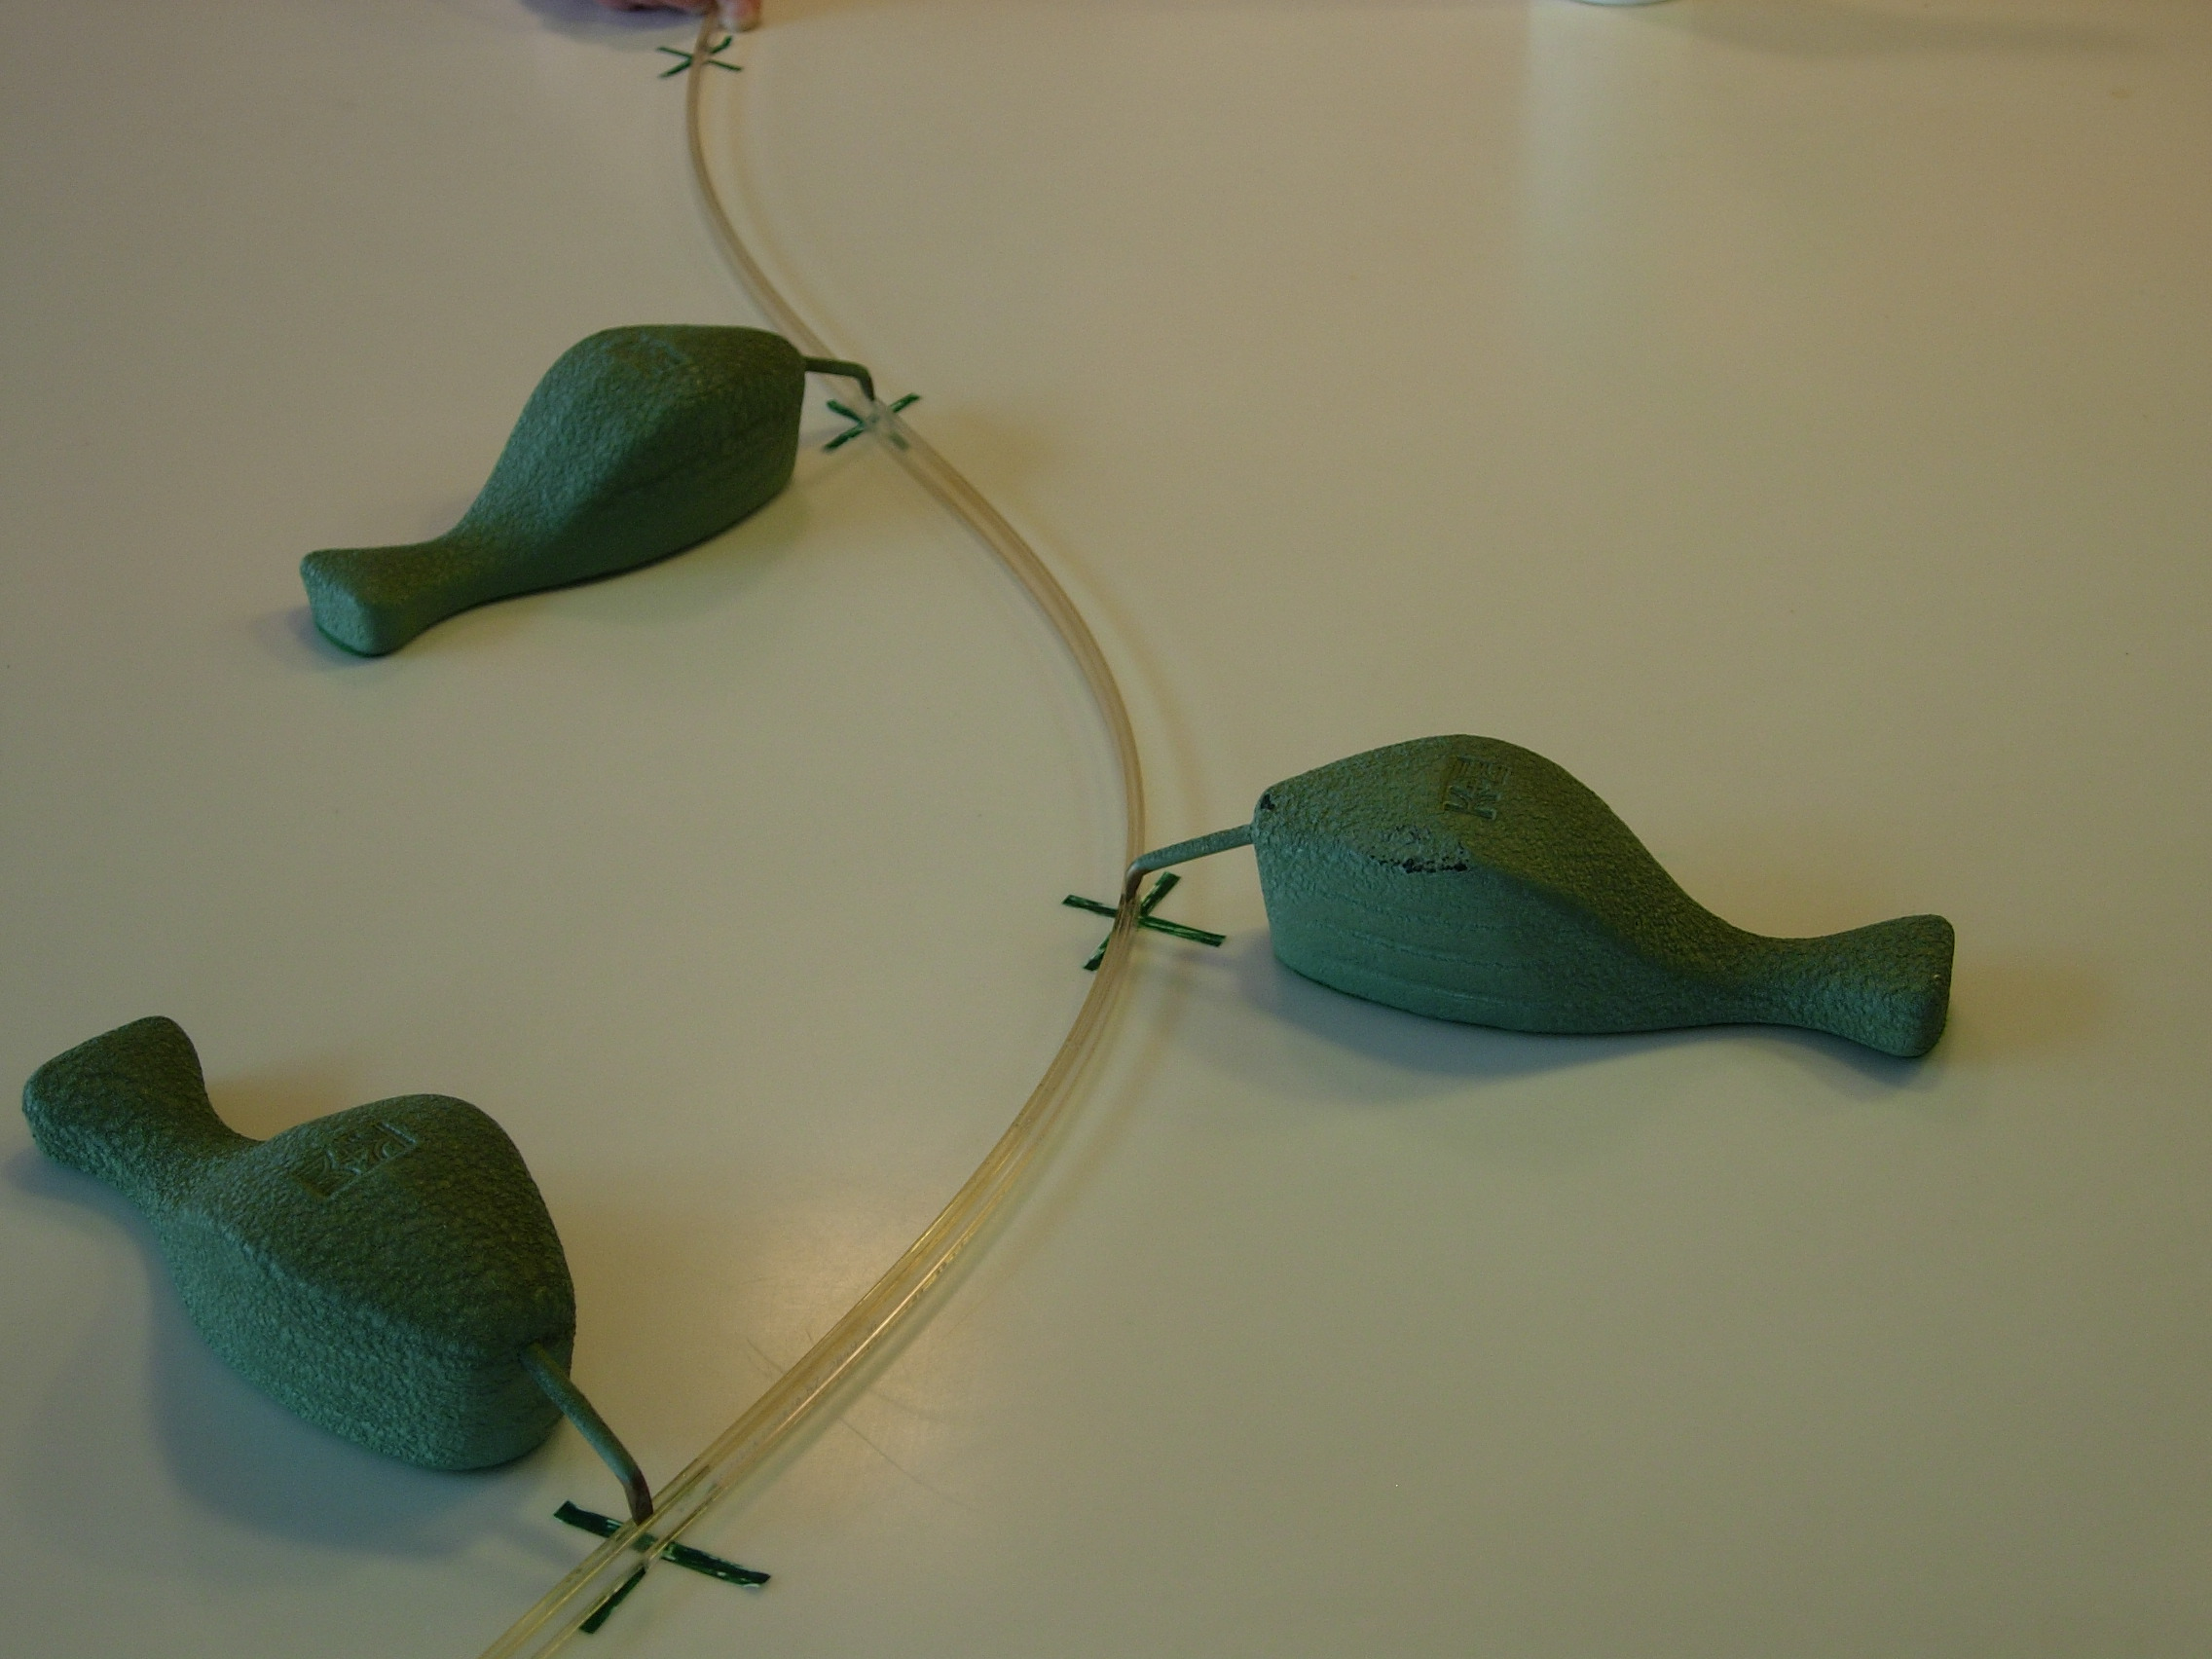
\includegraphics[width=0.49\textwidth]{figs/spline2.png}
\end{center}

\end{frame}

\begin{frame}[t]{Splines in 1d - Smoothing Splines}
\protect\hypertarget{splines-in-1d---smoothing-splines}{}

These are a mathematical analogue to the drafting splines represented
using a penalized regression model.

\pause

We want to find a function \(f(x)\) that best fits our observed data
\(\symbf{y} = y_1, \ldots, y_n\) while being as \emph{smooth} as
possible.

\[ \underset{f(x)}{\arg\min} ~ \sum_{i=1}^n\left(y_i - f(x_i)\right)^2 + \lambda \int_{-\infty}^\infty f''(x)^2 ~ dx \]

Interestingly, this minimization problem has an exact solution which is
given by a mixture of weighted natural cubic splines (cubic splines that
are linear in the tails) with knots at the observed data locations
(\(x\)s).

\end{frame}

\begin{frame}{Splines in 2d - Thin Plate Splines}
\protect\hypertarget{splines-in-2d---thin-plate-splines}{}

Now imagine we have observed data of the form \((x_i, y_i, z_i)\) where
we wish to predict \(z_i\) given \(x_i\) and \(y_i\) for all \(i\). We
can naturally extend the smoothing spline model in two dimensions,

\[ \underset{f(x,y)}{\arg\min} ~~ \sum_{i=1}^n (z_i-f(x_i,y_i))^2 + \lambda  \int_{-\infty}^\infty  \int_{-\infty}^\infty \left(\frac{\partial^2 f}{\partial x^2} + 2 \frac{\partial^2 f}{\partial x \, \partial y} + \frac{\partial^2 f}{\partial y^2} \right) dx\, dy\]

The solution to this equation has a natural representation using a
weighted sum of \emph{radial basis functions} with knots at the observed
data locations

\[ f(x,y) = \sum_{i=1}^n w_i ~ d(x_i,y_i)^2 \log d(x_i,y_i).  \]

\end{frame}

\begin{frame}[fragile,t]{Fitting a TPS}
\protect\hypertarget{fitting-a-tps}{}

\scriptoutput
\vspace{-7.5mm}

\begin{Shaded}
\begin{Highlighting}[]
\NormalTok{coords =}\StringTok{ }\KeywordTok{select}\NormalTok{(csn, }\DataTypeTok{long=}\NormalTok{longitude, }\DataTypeTok{lat=}\NormalTok{latitude) }\OperatorTok\StringTok{ }\KeywordTok{as.matrix}\NormalTok{()}
\NormalTok{tps =}\StringTok{ }\NormalTok{fields}\OperatorTok{::}\KeywordTok{Tps}\NormalTok{(}\DataTypeTok{x =}\NormalTok{ coords, }\DataTypeTok{Y=}\NormalTok{csn}\OperatorTok{$}\NormalTok{pm25)}


\KeywordTok{data}\NormalTok{(wrld_simpl, }\DataTypeTok{package =} \StringTok{"maptools"}\NormalTok{)}

\NormalTok{r =}\StringTok{ }\NormalTok{raster}\OperatorTok{::}\KeywordTok{raster}\NormalTok{(}\DataTypeTok{nrows=}\DecValTok{200}\NormalTok{, }\DataTypeTok{ncol=}\DecValTok{400}\NormalTok{,}
           \DataTypeTok{xmn =} \KeywordTok{min}\NormalTok{(csn}\OperatorTok{$}\NormalTok{longitude)}\OperatorTok{*}\FloatTok{1.05}\NormalTok{, }\DataTypeTok{xmx =} \KeywordTok{max}\NormalTok{(csn}\OperatorTok{$}\NormalTok{longitude)}\OperatorTok{*}\FloatTok{0.95}\NormalTok{,}
           \DataTypeTok{ymn =} \KeywordTok{min}\NormalTok{(csn}\OperatorTok{$}\NormalTok{latitude )}\OperatorTok{*}\FloatTok{0.95}\NormalTok{, }\DataTypeTok{ymx =} \KeywordTok{max}\NormalTok{(csn}\OperatorTok{$}\NormalTok{latitude )}\OperatorTok{*}\FloatTok{1.05}\NormalTok{)}

\NormalTok{usa =}\StringTok{ }\NormalTok{raster}\OperatorTok{::}\KeywordTok{rasterize}\NormalTok{(wrld_simpl[wrld_simpl}\OperatorTok{$}\NormalTok{NAME }\OperatorTok{==}\StringTok{ "United States"}\NormalTok{,], r)}

\NormalTok{cells =}\StringTok{ }\KeywordTok{which}\NormalTok{(}\OperatorTok{!}\KeywordTok{is.na}\NormalTok{(usa[]))}
\NormalTok{pred_coords =}\StringTok{ }\NormalTok{raster}\OperatorTok{::}\KeywordTok{xyFromCell}\NormalTok{(r, cells)}

\NormalTok{pm25_pred =}\StringTok{ }\NormalTok{r}
\NormalTok{pm25_pred[cells] =}\StringTok{ }\KeywordTok{predict}\NormalTok{(tps, pred_coords)}

\NormalTok{pm25_pred_df =}\StringTok{ }\KeywordTok{as}\NormalTok{(pm25_pred, }\StringTok{"SpatialPixelsDataFrame"}\NormalTok{) }\OperatorTok\StringTok{ }
\StringTok{  }\KeywordTok{as.data.frame}\NormalTok{() }\OperatorTok
\StringTok{  }\KeywordTok{select}\NormalTok{(}\DataTypeTok{long=}\NormalTok{x, }\DataTypeTok{lat=}\NormalTok{y, }\DataTypeTok{pm25 =}\NormalTok{ layer)}
\end{Highlighting}
\end{Shaded}

\end{frame}

\begin{frame}{}
\protect\hypertarget{section-3}{}

\begin{center}\includegraphics[width=\textwidth,height=\textheight]{Lec19_files/figure-beamer/unnamed-chunk-36-1} \end{center}

\end{frame}

\hypertarget{gaussin-process-models-kriging}{%
\section{Gaussin Process Models /
Kriging}\label{gaussin-process-models-kriging}}

\begin{frame}[fragile]{Variogram}
\protect\hypertarget{variogram}{}

\scriptoutput

\begin{Shaded}
\begin{Highlighting}[]
\NormalTok{coords =}\StringTok{ }\NormalTok{csn }\OperatorTok\StringTok{ }\KeywordTok{select}\NormalTok{(latitude, longitude) }\OperatorTok\StringTok{ }\KeywordTok{as.matrix}\NormalTok{()}
\NormalTok{d =}\StringTok{ }\NormalTok{fields}\OperatorTok{::}\KeywordTok{rdist}\NormalTok{(coords)}

\NormalTok{geoR}\OperatorTok{::}\KeywordTok{variog}\NormalTok{(}\DataTypeTok{coords =}\NormalTok{ coords, }\DataTypeTok{data =}\NormalTok{ csn}\OperatorTok{$}\NormalTok{pm25, }\DataTypeTok{messages =} \OtherTok{FALSE}\NormalTok{, }
       \DataTypeTok{uvec =} \KeywordTok{seq}\NormalTok{(}\DecValTok{0}\NormalTok{, }\KeywordTok{max}\NormalTok{(d)}\OperatorTok{/}\DecValTok{2}\NormalTok{, }\DataTypeTok{length.out=}\DecValTok{50}\NormalTok{)) }\OperatorTok\StringTok{ }\KeywordTok{plot}\NormalTok{()}
\end{Highlighting}
\end{Shaded}

\begin{center}\includegraphics[width=\textwidth]{Lec19_files/figure-beamer/unnamed-chunk-37-1} \end{center}

\end{frame}

\begin{frame}[fragile]{}
\protect\hypertarget{section-4}{}

\begin{Shaded}
\begin{Highlighting}[]
\NormalTok{geoR}\OperatorTok{::}\KeywordTok{variog}\NormalTok{(}\DataTypeTok{coords =}\NormalTok{ coords, }\DataTypeTok{data =}\NormalTok{ csn}\OperatorTok{$}\NormalTok{pm25, }\DataTypeTok{messages =} \OtherTok{FALSE}\NormalTok{,}
       \DataTypeTok{uvec =} \KeywordTok{seq}\NormalTok{(}\DecValTok{0}\NormalTok{, }\KeywordTok{max}\NormalTok{(d)}\OperatorTok{/}\DecValTok{4}\NormalTok{, }\DataTypeTok{length.out=}\DecValTok{50}\NormalTok{)) }\OperatorTok\StringTok{ }\KeywordTok{plot}\NormalTok{()}
\end{Highlighting}
\end{Shaded}

\begin{center}\includegraphics[width=\textwidth]{Lec19_files/figure-beamer/unnamed-chunk-38-1} \end{center}

\end{frame}

\begin{frame}[fragile]{Isotropy / Anisotropy}
\protect\hypertarget{isotropy-anisotropy}{}

\scriptoutput

\begin{Shaded}
\begin{Highlighting}[]
\NormalTok{v4 =}\StringTok{ }\NormalTok{geoR}\OperatorTok{::}\KeywordTok{variog4}\NormalTok{(}\DataTypeTok{coords =}\NormalTok{ coords, }\DataTypeTok{data =}\NormalTok{ csn}\OperatorTok{$}\NormalTok{pm25, }\DataTypeTok{messages =} \OtherTok{FALSE}\NormalTok{,}
             \DataTypeTok{uvec =} \KeywordTok{seq}\NormalTok{(}\DecValTok{0}\NormalTok{, }\KeywordTok{max}\NormalTok{(d)}\OperatorTok{/}\DecValTok{4}\NormalTok{, }\DataTypeTok{length.out =} \DecValTok{50}\NormalTok{))}
\KeywordTok{plot}\NormalTok{(v4)}
\end{Highlighting}
\end{Shaded}

\begin{center}\includegraphics[width=\textwidth]{Lec19_files/figure-beamer/unnamed-chunk-39-1} \end{center}

\end{frame}

\begin{frame}{GP Spatial Model}
\protect\hypertarget{gp-spatial-model}{}

\small

If we assume that our data is \emph{stationary} and \emph{isotropic}
then we can use a Gaussian Process model to fit the data. We will assume
an exponential covariance structure.

\[ \symbf{y} \sim \mathcal{N}(\symbf{\mu},~\Sigma) \]
\[ \{\Sigma\}_{ij} = \sigma^2 \exp(- r \, \lVert s_i - s_j\lVert) + \sigma^2_n \, 1_{i=j} \]

\pause

we can also view this as a spatial random effects model where

\[ y(\symbf{s}) = \mu(\symbf{s}) + w(\symbf{s}) + \epsilon(\symbf{s}) \]
\[ w(\symbf{s}) \sim \mathcal{N}(0,\Sigma') \]
\[ \epsilon(s_i) \sim \mathcal{N}(0,\sigma^2_n) \]
\[ \{\Sigma'\}_{ij} = \sigma^2 \exp(- r \, \lVert s_i - s_j\lVert) \]

\end{frame}

\begin{frame}[fragile,t]{Fitting with \texttt{spBayes}}
\protect\hypertarget{fitting-with-spbayes}{}

\begin{Shaded}
\begin{Highlighting}[]
\NormalTok{n =}\StringTok{ }\KeywordTok{nrow}\NormalTok{(csn)}
\NormalTok{n_samp =}\StringTok{ }\DecValTok{20000}
\NormalTok{coords =}\StringTok{ }\KeywordTok{select}\NormalTok{(csn, longitude, latitude) }\OperatorTok\StringTok{ }\KeywordTok{as.matrix}\NormalTok{()}
\NormalTok{max_range =}\StringTok{ }\KeywordTok{max}\NormalTok{(}\KeywordTok{dist}\NormalTok{(coords)) }\OperatorTok{/}\StringTok{ }\DecValTok{4}


\NormalTok{starting =}\StringTok{ }\KeywordTok{list}\NormalTok{(}\DataTypeTok{phi =} \DecValTok{3}\OperatorTok{/}\DecValTok{3}\NormalTok{, }\DataTypeTok{sigma.sq =} \DecValTok{33}\NormalTok{, }\DataTypeTok{tau.sq =} \DecValTok{17}\NormalTok{)}
\NormalTok{tuning =}\StringTok{ }\KeywordTok{list}\NormalTok{(}\StringTok{"phi"}\NormalTok{=}\FloatTok{0.1}\NormalTok{, }\StringTok{"sigma.sq"}\NormalTok{=}\FloatTok{0.1}\NormalTok{, }\StringTok{"tau.sq"}\NormalTok{=}\FloatTok{0.1}\NormalTok{)}
\NormalTok{priors =}\StringTok{ }\KeywordTok{list}\NormalTok{(}
  \DataTypeTok{beta.Norm =} \KeywordTok{list}\NormalTok{(}\DecValTok{0}\NormalTok{, }\DecValTok{1000}\NormalTok{), }
  \DataTypeTok{phi.Unif =} \KeywordTok{c}\NormalTok{(}\DecValTok{3}\OperatorTok{/}\NormalTok{max_range, }\DecValTok{3}\OperatorTok{/}\NormalTok{(}\FloatTok{0.5}\NormalTok{)), }
  \DataTypeTok{sigma.sq.IG =} \KeywordTok{c}\NormalTok{(}\DecValTok{2}\NormalTok{, }\DecValTok{2}\NormalTok{), }
  \DataTypeTok{tau.sq.IG =} \KeywordTok{c}\NormalTok{(}\DecValTok{2}\NormalTok{, }\DecValTok{2}\NormalTok{)}
\NormalTok{)}
\end{Highlighting}
\end{Shaded}

\end{frame}

\begin{frame}[fragile,t]{}
\protect\hypertarget{section-5}{}

\tinyoutput

\begin{Shaded}
\begin{Highlighting}[]
\NormalTok{m =}\StringTok{ }\NormalTok{spBayes}\OperatorTok{::}\KeywordTok{spLM}\NormalTok{(pm25 }\OperatorTok{~}\StringTok{ }\DecValTok{1}\NormalTok{, }\DataTypeTok{data =}\NormalTok{ csn, }\DataTypeTok{coords =}\NormalTok{ coords, }\DataTypeTok{starting =}\NormalTok{ starting, }\DataTypeTok{priors =}\NormalTok{ priors, }
         \DataTypeTok{cov.model =} \StringTok{"exponential"}\NormalTok{, }\DataTypeTok{n.samples =}\NormalTok{ n_samp, }\DataTypeTok{tuning =}\NormalTok{ tuning,}
         \DataTypeTok{n.report =}\NormalTok{ n_samp}\OperatorTok{/}\DecValTok{2}\NormalTok{)}
\CommentTok{## ----------------------------------------}
\CommentTok{##  General model description}
\CommentTok{## ----------------------------------------}
\CommentTok{## Model fit with 191 observations.}
\CommentTok{## }
\CommentTok{## Number of covariates 1 (including intercept if specified).}
\CommentTok{## }
\CommentTok{## Using the exponential spatial correlation model.}
\CommentTok{## }
\CommentTok{## Number of MCMC samples 20000.}
\CommentTok{## }
\CommentTok{## Priors and hyperpriors:}
\CommentTok{##  beta normal:}
\CommentTok{##  mu: 0.000   }
\CommentTok{##  cov:}
\CommentTok{##  1000.000    }
\CommentTok{## }
\CommentTok{##  sigma.sq IG hyperpriors shape=2.00000 and scale=2.00000}
\CommentTok{##  tau.sq IG hyperpriors shape=2.00000 and scale=2.00000}
\CommentTok{##  phi Unif hyperpriors a=0.21888 and b=6.00000}
\CommentTok{## -------------------------------------------------}
\CommentTok{##      Sampling}
\CommentTok{## -------------------------------------------------}
\CommentTok{## Sampled: 10000 of 20000, 50.00%}
\CommentTok{## Report interval Metrop. Acceptance rate: 32.56%}
\CommentTok{## Overall Metrop. Acceptance rate: 32.56%}
\CommentTok{## -------------------------------------------------}
\CommentTok{## Sampled: 20000 of 20000, 100.00%}
\CommentTok{## Report interval Metrop. Acceptance rate: 32.82%}
\CommentTok{## Overall Metrop. Acceptance rate: 32.69%}
\CommentTok{## -------------------------------------------------}
\end{Highlighting}
\end{Shaded}

\end{frame}

\begin{frame}[fragile,t]{}
\protect\hypertarget{section-6}{}

\scriptoutput

\begin{Shaded}
\begin{Highlighting}[]
\NormalTok{m =}\StringTok{ }\NormalTok{spBayes}\OperatorTok{::}\KeywordTok{spRecover}\NormalTok{(m, }\DataTypeTok{start=}\NormalTok{n_samp}\OperatorTok{/}\DecValTok{2}\OperatorTok{+}\DecValTok{1}\NormalTok{, }\DataTypeTok{thin =}\NormalTok{ (n_samp}\OperatorTok{/}\DecValTok{2}\NormalTok{)}\OperatorTok{/}\DecValTok{1000}\NormalTok{)}
\CommentTok{## -------------------------------------------------}
\CommentTok{##      Recovering beta and w}
\CommentTok{## -------------------------------------------------}
\CommentTok{## Sampled: 99 of 1000, 9.90%}
\CommentTok{## Sampled: 199 of 1000, 19.90%}
\CommentTok{## Sampled: 299 of 1000, 29.90%}
\CommentTok{## Sampled: 399 of 1000, 39.90%}
\CommentTok{## Sampled: 499 of 1000, 49.90%}
\CommentTok{## Sampled: 599 of 1000, 59.90%}
\CommentTok{## Sampled: 699 of 1000, 69.90%}
\CommentTok{## Sampled: 799 of 1000, 79.90%}
\CommentTok{## Sampled: 899 of 1000, 89.90%}
\CommentTok{## Sampled: 999 of 1000, 99.90%}
\end{Highlighting}
\end{Shaded}

\end{frame}

\begin{frame}[fragile]{Parameter values}
\protect\hypertarget{parameter-values}{}

\begin{Shaded}
\begin{Highlighting}[]
\NormalTok{theta =}\StringTok{ }\NormalTok{m}\OperatorTok{$}\NormalTok{p.theta.recover.samples }\OperatorTok
\StringTok{  }\NormalTok{tidybayes}\OperatorTok{::}\KeywordTok{gather_samples}\NormalTok{(sigma.sq, tau.sq, phi)}
\end{Highlighting}
\end{Shaded}

\begin{center}\includegraphics[width=\textwidth]{Lec19_files/figure-beamer/unnamed-chunk-44-1} \end{center}

\end{frame}

\begin{frame}[fragile]{}
\protect\hypertarget{section-7}{}

\begin{Shaded}
\begin{Highlighting}[]
\NormalTok{m}\OperatorTok{$}\NormalTok{p.beta.recover.samples }\OperatorTok
\StringTok{  }\NormalTok{tidybayes}\OperatorTok{::}\KeywordTok{gather_samples}\NormalTok{(}\StringTok{`}\DataTypeTok{(Intercept)}\StringTok{`}\NormalTok{) }\OperatorTok
\StringTok{  }\KeywordTok{ggplot}\NormalTok{(}\KeywordTok{aes}\NormalTok{(}\DataTypeTok{x=}\NormalTok{.iteration, }\DataTypeTok{y=}\NormalTok{estimate, }\DataTypeTok{color=}\NormalTok{term)) }\OperatorTok{+}
\StringTok{    }\KeywordTok{geom_line}\NormalTok{() }\OperatorTok{+}
\StringTok{    }\KeywordTok{facet_grid}\NormalTok{(term}\OperatorTok{~}\NormalTok{., }\DataTypeTok{scales =} \StringTok{"free_y"}\NormalTok{) }\OperatorTok{+}
\StringTok{    }\KeywordTok{guides}\NormalTok{(}\DataTypeTok{color=}\OtherTok{FALSE}\NormalTok{)}
\end{Highlighting}
\end{Shaded}

\begin{center}\includegraphics[width=\textwidth]{Lec19_files/figure-beamer/unnamed-chunk-45-1} \end{center}

\end{frame}

\begin{frame}[fragile]{Predictions}
\protect\hypertarget{predictions-2}{}

\tinyoutput

\begin{Shaded}
\begin{Highlighting}[]
\NormalTok{m_pred =}\StringTok{ }\NormalTok{spBayes}\OperatorTok{::}\KeywordTok{spPredict}\NormalTok{(m, pred_coords, }\DataTypeTok{pred.covars =} \KeywordTok{matrix}\NormalTok{(}\DecValTok{1}\NormalTok{, }\DataTypeTok{nrow=}\KeywordTok{nrow}\NormalTok{(pred_coords)), }
                   \DataTypeTok{start=}\NormalTok{n_samp}\OperatorTok{/}\DecValTok{2}\OperatorTok{+}\DecValTok{1}\NormalTok{, }\DataTypeTok{thin=}\NormalTok{(n_samp}\OperatorTok{/}\DecValTok{2}\NormalTok{)}\OperatorTok{/}\DecValTok{1000}\NormalTok{)}
\CommentTok{## ----------------------------------------}
\CommentTok{##  General model description}
\CommentTok{## ----------------------------------------}
\CommentTok{## Model fit with 191 observations.}
\CommentTok{## }
\CommentTok{## Prediction at 900 locations.}
\CommentTok{## }
\CommentTok{## Number of covariates 1 (including intercept if specified).}
\CommentTok{## }
\CommentTok{## Using the exponential spatial correlation model.}
\CommentTok{## }
\CommentTok{## -------------------------------------------------}
\CommentTok{##      Sampling}
\CommentTok{## -------------------------------------------------}
\CommentTok{## Sampled: 100 of 1000, 9.90%}
\CommentTok{## Sampled: 200 of 1000, 19.90%}
\CommentTok{## Sampled: 300 of 1000, 29.90%}
\CommentTok{## Sampled: 400 of 1000, 39.90%}
\CommentTok{## Sampled: 500 of 1000, 49.90%}
\CommentTok{## Sampled: 600 of 1000, 59.90%}
\CommentTok{## Sampled: 700 of 1000, 69.90%}
\CommentTok{## Sampled: 800 of 1000, 79.90%}
\CommentTok{## Sampled: 900 of 1000, 89.90%}
\CommentTok{## Sampled: 1000 of 1000, 99.90%}
\NormalTok{m_pred_summary =}\StringTok{ }\KeywordTok{post_summary}\NormalTok{(}\KeywordTok{t}\NormalTok{(m_pred}\OperatorTok{$}\NormalTok{p.y.predictive.samples))}
\end{Highlighting}
\end{Shaded}

\end{frame}

\begin{frame}{}
\protect\hypertarget{section-8}{}

\begin{center}\includegraphics[width=\textwidth]{Lec19_files/figure-beamer/unnamed-chunk-48-1} \end{center}

\end{frame}

\begin{frame}[fragile]{JAGs Model}
\protect\hypertarget{jags-model}{}

\begin{Shaded}
\begin{Highlighting}[]
\NormalTok{gplm =}\StringTok{ "model\{}
\StringTok{  for(i in 1:length(y))\{}
\StringTok{    y[i] ~ dnorm(beta + w[i], tau)}
\StringTok{    mu_w[i] = 0}
\StringTok{  \}}
\StringTok{ }
\StringTok{  for(i in 1:length(y))\{}
\StringTok{    for(j in 1:length(y))\{}
\StringTok{      Sigma_w[i,j] = sigma2_w * exp(-phi * d[i,j])}
\StringTok{    \}}
\StringTok{  \}}
\StringTok{  w ~ dmnorm(mu_w, inverse(Sigma_w))}

\StringTok{  beta ~ dnorm(0, 1/1000)}
\StringTok{  sigma2_w ~ dgamma(2, 2)}
\StringTok{  sigma2 ~ dgamma(2, 2)}
\StringTok{  tau = 1/sigma2}
\StringTok{  phi ~ dunif(3/14, 3/0.5)}
\StringTok{\}"}
\end{Highlighting}
\end{Shaded}

\end{frame}

\begin{frame}{}
\protect\hypertarget{section-9}{}

\begin{center}\includegraphics[width=\textwidth]{Lec19_files/figure-beamer/unnamed-chunk-50-1} \end{center}

\end{frame}

\begin{frame}{Comparing Model Parameters}
\protect\hypertarget{comparing-model-parameters}{}

\begin{center}\includegraphics[width=\textwidth]{Lec19_files/figure-beamer/unnamed-chunk-51-1} \end{center}

\end{frame}

\end{document}
